%%%%%%%%%%%%%%%%%%%%%%%%%%%%%%%%%%%%%%%%%%%%%%%%%%%%%%%%%%%%%%%%%%%%%%%%%%%%%%
%%%%%%%%%%%%%%%%%%%%%%%%%%%%%%%%%%%%%%%%%%%%%%%%%%%%%%%%%%%%%%%%%%%%%%%%%%%%%%
%%
%% Ukázkový příklad dokumentace úkolu do předmětů IZP a IUS, 2010
%%
%% Upravená původní dokumentace od Davida Martinka.
%%%%%%%%%%%%%%%%%%%%%%%%%%%%%%%%%%%%%%%%%%%%%%%%%%%%%%%%%%%%%%%%%%%%%%%%%%%%%%
%%%%%%%%%%%%%%%%%%%%%%%%%%%%%%%%%%%%%%%%%%%%%%%%%%%%%%%%%%%%%%%%%%%%%%%%%%%%%%
\documentclass[12pt,a4paper,titlepage,final]{article}

% cestina a fonty
\usepackage[english]{babel}
\usepackage[utf8]{inputenc}



% balicky pro odkazy
\usepackage[colorlinks,plainpages=false,urlcolor=blue,unicode]
{hyperref}
\usepackage{url}
% obrazky
\usepackage[dvipdf]{graphicx}

% velikost stranky
\usepackage[top=3.5cm, left=2.5cm, text={17cm, 24cm}, ignorefoot]{geometry}

% fixne footnote stale dole na stranke
\usepackage[bottom]{footmisc}
% kvoli nazvom tried a funkcii
\usepackage{courier}
\usepackage{svg}
\usepackage{float}

\begin{document}

%%%%%%%%%%%%%%%%%%%%%%%%%%%%%%%%%%%%%%%%%%%%%%%%%%%%%%%%%%%%%%%%%%%%%%%%%%%%%%
% titulní strana

% !!!!!!!!!!!!!!!!!!!!!!!!!!!!!!!!!!!!!!!!!!!!!!!!!
% změň následující údaje za své
\def\myauthor{Ladislav Šulák}
\def\myauthorA{Krisztián Benko}
%\def\mycoauthor{Samuel Jaklovský} 
\def\myemail{xsulak04@stud.fit.vutbr.cz}
\def\myemailA{kristianbnk@gmail.com}
%\def\mycoemail{xjaklo02@stud.fit.vutbr.cz}
\def\projname{Fuzzy string searching}
% !!!!!!!!!!!!!!!!!!!!!!!!!!!!!!!!!!!!!!!!!!!!!!!!!

% !TeX spellcheck = en_US
\begin{titlepage}

% \vspace*{1cm}
\begin{figure}[!h]
  \centering
  
\includegraphics[height=4cm, width = 16cm]{img/logo-tei-crete.png}
\end{figure}

\vfill

\begin{center}
\begin{Large}
Third project to subject Computational Intelligence\\
\end{Large}
\bigskip
\begin{Huge}
\projname\\
\end{Huge}

\end{center}

\vfill

\begin{center}
\begin{Large}
\today
\end{Large}
\end{center}

\vfill

\begin{flushleft}
\begin{large}
\begin{tabular}{ll}
Authors: & \myauthor, \url{\myemail} \\
& \myauthorA, \url{\myemailA} \\
%& \mycoauthor, \url{\mycoemail} \\
\end{tabular}
\end{large}
\end{flushleft}
\end{titlepage}


%%%%%%%%%%%%%%%%%%%%%%%%%%%%%%%%%%%%%%%%%%%%%%%%%%%%%%%%%%%%%%%%%%%%%%%%%%%%%%
% obsah
\pagestyle{plain}
\pagenumbering{roman}
\setcounter{page}{1}
\tableofcontents

%%%%%%%%%%%%%%%%%%%%%%%%%%%%%%%%%%%%%%%%%%%%%%%%%%%%%%%%%%%%%%%%%%%%%%%%%%%%%%
% textova zprava
\newpage
\pagestyle{plain}
\pagenumbering{arabic}
\setcounter{page}{1}

%%%%%%%%%%%%%%%%%%%%%%%%%%%%%%%%%%%%%%%%%%%%%%%%%%%%%%%%%%%%%%%%%%%%%%%%%%%%%%
\section{Introduction} \label{intro}
%%%%%%%%%%%%%%%%%%%%%%%%%%%%%%%%%%%%%%%%%%%%%%%%%%%%%%%%%%%%%%%%%%%%%%%%%%%%%%
This documentation describes a design and a development of a simple tool which utilizes the fuzzy string searching. Following aspects of the development will be described: problem analysis, design and implementation of the final application and benchmark tests along with proposal improvements or ideas. The aim of this project was to create an application, which could find a given string with some typo in a given input text.

The report is conceived as follows: in Section \ref{analysis} we describe the main points of our assignment such as the motivation and background along with some details about the project and its steps. In next Section \ref{design} we will  describe how we approached to this problem and there are also details about the algorithm we created. In Section \ref{impl} we describe our tool from implementation point of view in more details. Section \ref{test} deals with testing and benchmarking on a dataset we chose. Last Section \ref{conclusion} summaries this work.

\newpage

%%%%%%%%%%%%%%%%%%%%%%%%%%%%%%%%%%%%%%%%%%%%%%%%%%%%%%%%%%%%%%%%%%%%%%%%%%%%%%
\section{Analysis} \label{analysis}
%%%%%%%%%%%%%%%%%%%%%%%%%%%%%%%%%%%%%%%%%%%%%%%%%%%%%%%%%%%%%%%%%%%%%%%%%%%%%%
The main requirement of this project was to implement an application, which involves fuzzy logic and also to choose a dataset for the input of this application. So first we had to do a research to find out what possible applications based on fuzzy logic are. After that, we decided what will be the input and how we will get the dataset. The whole project can be decomposed to few separated tasks we were dealing with.

	\subsection{Groundwork}
	Firstly we were looking for a number suitable real-world applications with the usage of fuzziness and then we picked one. Our choice was a simple tool which could match searched pattern in the text approximately rather than exactly. String searching algorithm can be used for working with human alphabet ($\Sigma$ is for example in range from $a$ to $z$) or DNA alphabet ($\Sigma = \{A,C,G,T\}$). Approximate string searching can be a base for various applications related to spell checking, matching the nucleotide sequence in DNA data or spam filtering. String matching for binary data is not suitable since it fits better for different algorithms which are more optimal for such problem.

	The closeness of the approximate match between two strings is measured by the number of certain operations needed for converting a given string to another one. The usual operations are insertion, deletion and substitution, but some algorithms can also use another operations, like transposition. The computation of the difference between two strings is based on these operations and it is often called Levenshtein distance, or a more general, an edit distance.

	There are many such algorithms in the wild (see \cite{approximate} and \cite{substring}) and we used Bitap (Baeza-Yates–Gonnet) algorithm \cite{bitap2}. It can have 2 variants, a one for exact and a one for approximate string searching. We chose a latter one. It uses only substitution operation, which is a similar when a person do a typo error during writing and strikes a bit different key. This algorithms consider 2 strings to be equal if the number of such errors is within a given distance $k$ of each other. In other words, a Hamming distance of $k$. The algorithm begins with pre-computing a set of bitmasks containing one bit for each element from a given pattern. Then it utilizes a bitwise operations, which are extremely fast. It is used in a well-known Unix tool agrep (approximate grep).

	\subsection{Dataset} \label{dataset}
	The next part of the project's assignment was to find out the suitable data for our application mostly for testing the correctness of a solution. As a data source, we will e-book The Project Gutenberg e-book of The Adventures of Sherlock
Holmes written by Sir Arthur Conan Doyle extended by some other words and sentences. It has more than 6,4 millions of characters and more than 80,000 non-empty lines. For testing and evaluation, we need pairs consisting always from a given searched pattern (consisting 0 or more typos created by substitution of 2 letters) and text in which we could find a given pattern or a similar one. From a given data source, it would be good to extract lines. Each line would represent a text as a  searched area and from it we would randomly choose one word which would represent a searched pattern. With usage of pseudo-randomness, we would generate a typos and we could evaluate not only correctness of our solution, but also the average time when different number of typos are present in our dataset as well as a different lengths of a patterns or a searched text.

	\subsection{Decomposition of the project}
	The whole project from our perspective was broken down into following parts:
	\begin{enumerate}
		\item Find suitable application
		\item Define the data
   		 \item Presentation of the previous two steps
		\item Create a software design of the application
		\item Implement the application 
    	\item Experimentation, testing and benchmarking
    	\item The results and their analysis
    	\item Presentation of the final application and outcomes
    	\item This final report
	\end{enumerate}


%=============================================================================
\section{Design}  \label{design}
%=============================================================================
In this section we will briefly describe a design of the final application. It consist of a script which generates data from the dataset mentioned in the previous section. Regarding pseudo-randomness, it is very likely that each run the data will be a slightly different. We implemented both exact and approximate string matcher. Both have implemented various features for string searching and the implementation is in the same programming language written without the 3rd party libraries. It is ready for outputting a given result from the given parameters also on a bigger dataset.



%=============================================================================
\section{Implementation} \label{impl}
In this section we are going to describe the implementation of the application. For implementation purposes we chose to write in the Windows environment of PyCharm studio. We chose Python 3.6 programming language. We implemented a set of functions upon a given class containing Naive and Fuzzy searching. The functions are to find first match of the pattern, to find all the matches and to mark all patterns in a given text. Then, fuzzy checker is able to perform spell checker which corrects a given pattern based on a given text, so there is no other dictionary. The project structure is very simple, it contains just two scripts, one for data extraction and its manipulation and second for string matching:
	\begin{itemize}
		\item \textit{big.txt} - it contains English e-book written by Sir Arthur Conan Doyle as a dataset (see \ref{dataset} for more details),
		\item \textit{prepare\_data.py} - script for data extraction and processing, and
		\item \textit{fuzzy\_string\_matcher.py} - main script which utilizes a previous one and performs naive and fuzzy string matching along with spell correcting. 
	\end{itemize}

The application can be run with following arguments: printing help, finding all occurrences of the input pattern, marking all occurrences of the pattern or performing a spell check, respectively:

\texttt{fuzzy\_string\_matcher.py [-h] [--find\_all] [--mark\_all] [-spell\_check]}

The pseudo-code of Bitap algorithm for approximate matching\footnote{Our Bitap implementation was inspirated by \cite{bitap}} is depicted on Figure \ref{fig:bitap}.

\begin{figure}[H]
	\centering
	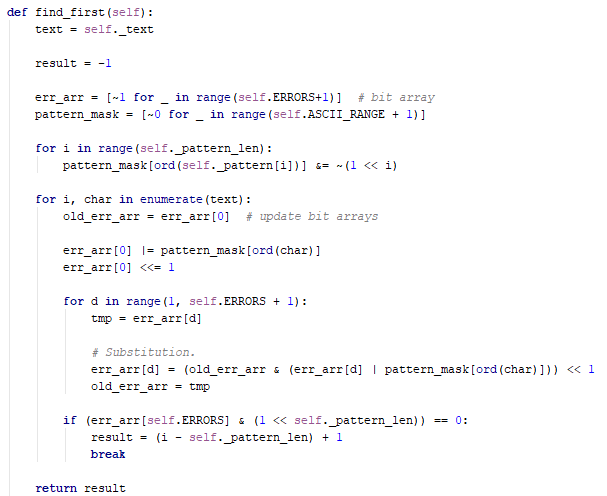
\includegraphics[height=11cm,keepaspectratio]{img/bitap.png}
	\caption{The pseudo-code of a Bitap algorithm which performs an approximate search by returning the first occurrence of the pattern's position in the input text.}
	\label{fig:bitap}
\end{figure}

Except Bitap algorithm, we also implemented Naive Pattern Searching algorithm\footnote{Our Naive Pattern Searching algorithm was mostly inspirated by \cite{naive}} which pseudo-code can be seen on Figure \ref{fig:naive}. It cycles an input text a letter by letter and it searches for the same beginning of a searched word. It should be noted, that there exist faster algorithms regarding exact string matching like KMP (Knuth–Morris–Prat), but further details out of the scope of this work. 

\begin{figure}[H]
	\centering
	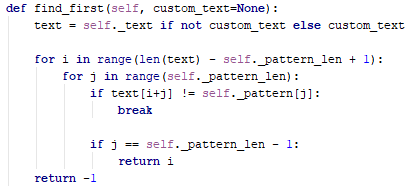
\includegraphics[height=4cm,keepaspectratio]{img/naive.png}
	\caption{The pseudo-code of a Naive String Searching algorithm which performs an exact search by returning the first occurrence of the pattern's position in the input text.}
	\label{fig:naive}
\end{figure}


\section{Experiments and benchmarking} \label{test}
Benchmark tests were performed on 25,000 pairs of (word, text), where:
	\begin{itemize}
		\item word is a searched word of size between 4 and 31 letters (6,6 in average),
		\item text contain at least 3 words and it is a searched area which always
contains words in English written correctly (121,1 letters in average)
	\end{itemize}

Each resulting runtime was calculated by performing 5 runs and then we calculated the average runtime. Dataset was generated automatically with pseudo-random generator (normal distribution) and some pairs can be duplicated. 

Firstly, we wanted to compare runtime of exact string matching (which means noise level was 0). Searching for all occurrences on our dataset took:
	\begin{itemize}
		\item \textit{FuzzyStringMatcher}: 4,7409755229949952 seconds
		\item \textit{NaiveStringMatcher}: 1,73054976463317872 seconds
	\end{itemize}
	
Then we measured the runtime of a different noise levels of our implementation of Bitap algorithm. It was growing linearly as we can see on Figure \ref{fig:bitap-noise-level}.

\begin{figure}[H]
	\centering
	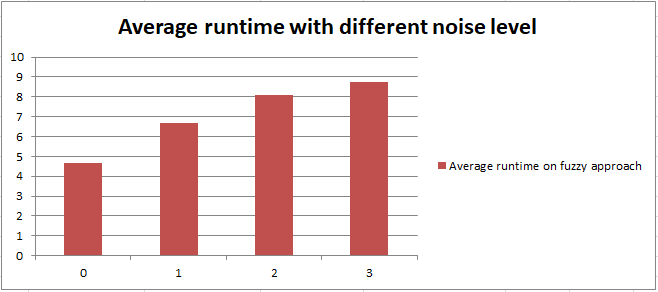
\includegraphics[height=5cm,keepaspectratio]{img/bitap-noise-graph.png}
	\caption{Bitap runtime measurement with a different number of typos. Each column represents the average CPU time calculated from five runs.}
	\label{fig:bitap-noise-level}
\end{figure}


\section{Conclusion} \label{conclusion}
The aim of this project was to find, design and to implement a practical application with the usage of fuzzy logic. We chose a approximate string searching also known as fuzzy string searching or matching. Firstly, we created a python script, which generates testing dataset for us pseudo-randomly. Final data contains always a pattern with zero or more typos and a segment of English text containing also at least one occurrence of a given pattern. Then we implemented a small tool for performing searching. The outcomes and achievements of our work are following:
	\begin{itemize}
		\item both exact (naive) and approximate (fuzzy) matching:
			\begin{itemize}
 				\item finding a position of a first occurrence of a searched word in a given text,
 				\item finding all the positions of occurrences of a searched word in a given text,
				\item marking all found words from a given text
			\end{itemize} 	
		\item spell corrector (only fuzzy approach):
 			\begin{itemize}
 				\item corrects an input word if there is a typo - substitution of a letter/s by another one/s, and
				\item correction is based on a given text (not external dictionary).
			\end{itemize} 	
	\end{itemize}

It showed, that time needed for computation is increasing with the number of typos and also that our naive string matcher was faster than our fuzzy string matcher. Since implementation language was chosen Python, which is language being interpreted rather than compiled, maybe the full potential of Bitap algorithm was not fully utilized. Even though, the asymptotic complexity of both algorithms is linear, but Bitap algorithm requires some preprocessing time (also linear).

Bitap, or some other approximate string searching algorithm, can be a base for applications regarding spam filtering, spell checking of some human language, or matching nucleotide sequence of DNA data as a heuristic method. 

\newpage

%\makeatletter
%\def\@openbib@code{\addcontentsline{toc}{chapter}{Bibliography}}
%\makeatother
\bibliographystyle{plain}
\bibliography{mybib}

\end{document}
